\documentclass{protokoll}
\newcommand{\assistent}{Dr. U. Blum}
\newcommand{\versuch}{Photoelektrische Bestimmung des Planckschen Wirkungsquantums}

\begin{document}

\section{Einleitung}
Der Photolektrische Effekt war schon einige Jahrzehnte bekannt bevor seine physikalische Erkl�rung schlie�lich durch \textsc{Einstein} im Jahre 1905 gelang. Sehr eindrucksvoll kann mit Hilfe dieses Experimentes die Quantelung der Energie elektromagnetischer Strahlung belegt werden.

\subsection{Photoelektrischer Effekt}
\label{cha:effekt}


\begin{figure}[h]
\centering
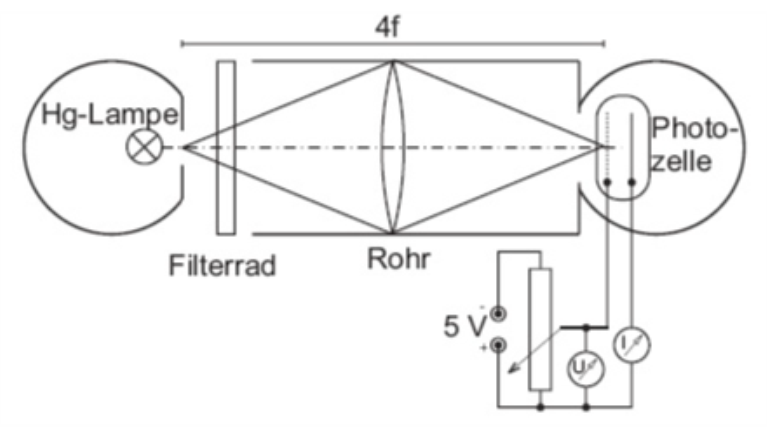
\includegraphics[width=0.6\textwidth]{aufbau}
\caption[Versuchsaufbau]{Versuchsaufbau zur Bestimmung des \textsc{Planck}schen Wirkungsquantums $h$. [2].}
\label{fig:aufbau}
\end{figure}



Die Energiebilanz f�r ein Elektron, welches durch ein Photon der Frequenz $\nu$ ausgel�st werden soll, ist durch die \textsc{Einstein}-Gleichung gegeben.

\begin{equation}
E_{kin} = h \nu - W_A
\end{equation}

Sobald also die Frequenz und somit die Energie des einfallenden Photons gro� genug ist, um $h \nu > W_A$ zu erf�llen, ist es in der Lage, das Elektron auszul�sen. �bersch�ssige Energie liegt anschlie�end in Form kinetischer Energie des Elektrons vor.


\subsection{Photozelle}
\label{cha:zelle}
Eine Photozelle (siehe Abb. \ref{fig:zelle}) ist zum Nachweis von Licht geeignet und besteht im Wesentlichen aus einem evakuierten Glaskolben und zwei Elektroden, der Anode und der Kathode.

\begin{figure}[h]
\centering
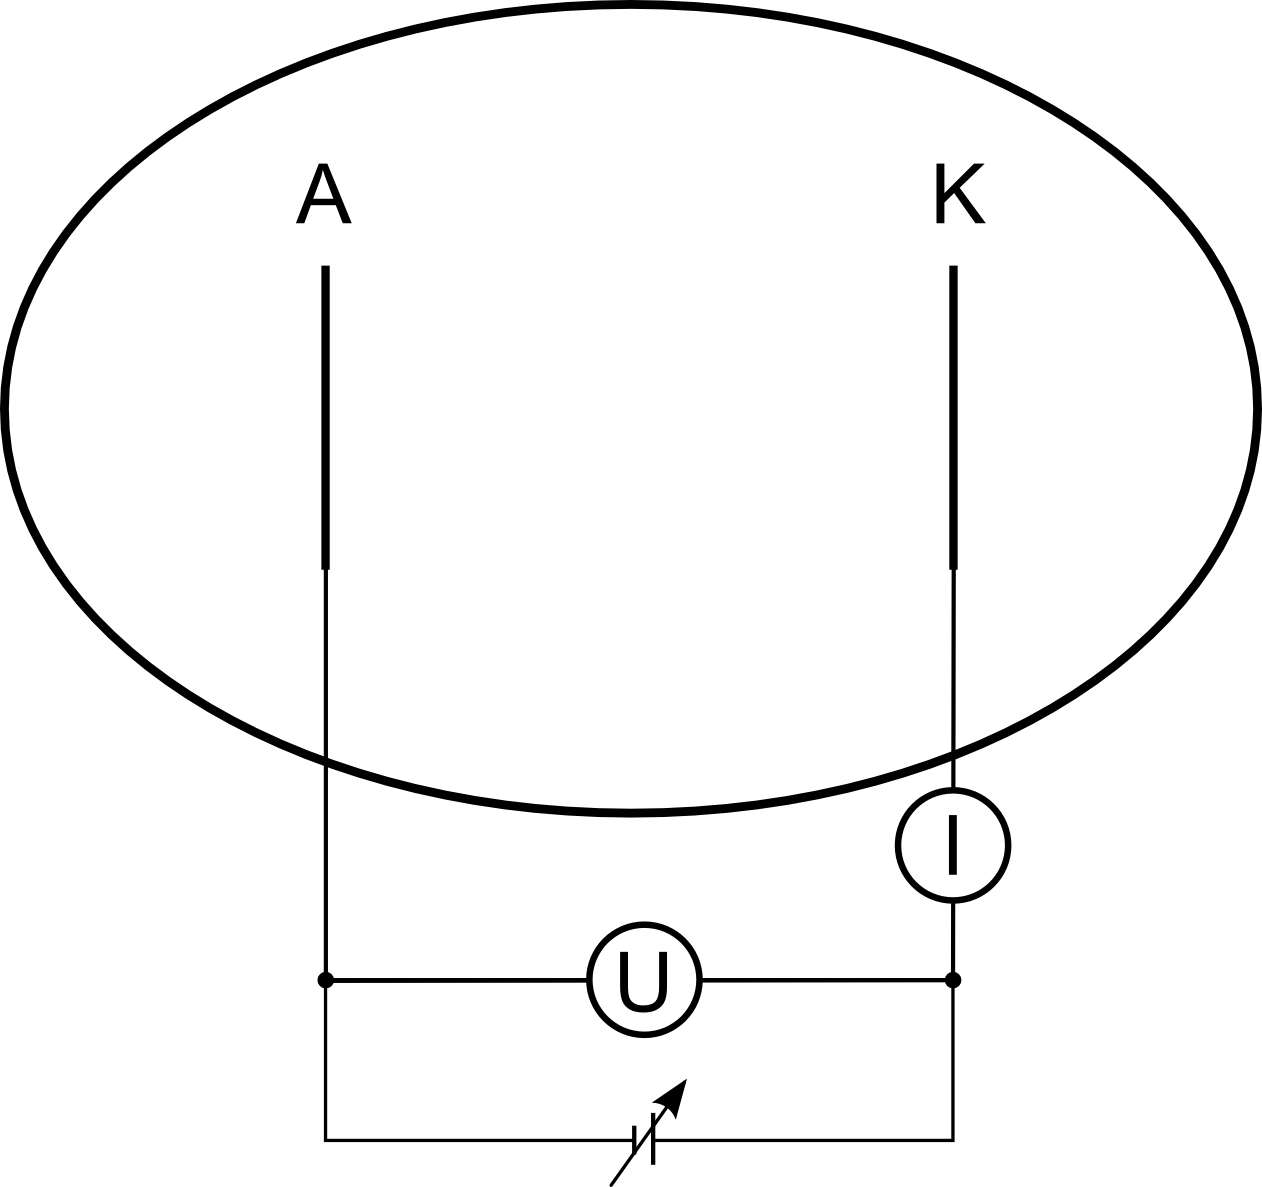
\includegraphics[width=0.6\textwidth]{zelle}
\caption[Photozelle]{Aufbau einer Photozelle.}
\label{fig:zelle}
\end{figure}

W�hrend die Kathode Elektronen bereitstellt, sammelt die Anode diese ein. Die Kathode ist aus einem Metall (z. B. C�sium) gefertigt und i.\ a.\ gro�fl�chiger angelegt, damit mehr Photonen auftreffen k�nnen. Die Anode hingegen ist meist als Drahtring realisiert, da hier m�glichst wenig Licht auftreffen soll. Des Weiteren ist die Austrittsarbeit der Anode oft h�her als die der Kathode. Diese beiden Umst�nde sorgen daf�r, dass die Anode im Wesentlichen nur absorbiert.

Es existieren zwei Betriebsm�glichkeiten. Entweder wird mit einer Saug- oder mit einer Gegenspannung gearbeitet. Im ersten Fall wird die Anode auf ein positives und die Kathode auf ein negatives Potential gesetzt (durch eine externe Spannungsquelle). Auf diese Weise werden die vom Licht an der Kathode freigesetzten Elektronen in Richtung der Anode beschleunigt. Es kann dann ein Anodenstrom (auftreffende Elektronen) gemessen werden.
Bei Betrieb mit Gegenspannung hingegen wird die Anode auf ein negativeres Potential als die Kathode gesetzt, so dass die Elektronen sich nach dem Verlassen der Kathode einem Gegenfeld ausgesetzt sehen, welches sie wieder in Richtung der Kathode beschleunigt. W�hlt man eine regelbare Gegenspannung, so kann auf diese Weise die kinetische Energie der Elektronen festgestellt werden (siehe \ref{cha:effekt}).


\subsection{Austrittsarbeit}
\label{cha:austritt}
Liegt ein einzelnes Atom vor, so bedarf die Ausl�sung eines Elektrons aus dem Atom eines Energie�bertrags an das Elektron, welcher der (gequantelten) Bindungsenergie entspricht. Nur bestimmte, diskrete Energiebetr�ge kommen dabei in Frage. Sobald jedoch mehrere Atome, beispielsweise in einem Festk�rper zu betrachten sind, liegen auf Grund der Wechselwirkungen zwischen den Atomen keine diskreten Bindungsenergien mehr vor. Vielmehr k�nnen die einzelnen Energieniveaus des Festk�rpers als verschmierte B�nder approximiert werden (B�ndermodell). Innerhalb dieser B�nder ergibt sich ein kontinuierlicher Energieverlauf. Jenes Energieband, welches dabei f�r $T = \unit[0]{K}$ �ber dem h�chsten mit Elektronen vollst�ndig besetzten Energieband (Valenzband) liegt, bezeichnet man i.\ a.\ als Leitungsband. Im Leitungsband befindliche Elektronen sind im Gegensatz zu denen im Valenzband frei beweglich, d.h. sie lassen sich nicht mehr einzelnen Atomr�mpfen zuordnen, sondern nur noch dem Festk�rper als ganzem.
Als Austrittsarbeit $W_A$ bezeichnet man nun den zur Ausl�sung eines Elektrons aus einem elektrisch neutralen Festk�rper mindestens notwendigen Energiebetrag. Insbesondere ist die Austrittsarbeit dabei f�r alle im Leitungsband befindlichen Elektronen identisch, in Abgrenzung zu den Bindungsenergien der Elektronen aus verschiedenen Elektronenschalen im einzelnen Atom.
Offenbar ist also je nach Besetzung der B�nder, also je nach Lage des \textsc{Fermi}-Niveaus eine unterschiedliche Austrittsarbeit $W_A$ zu leisten. $W_A$ ist demnach somit eine Materialeigenschaft.

Im vorliegenden Fall sollen Photonen die Energie bereitstellen, um Elektronen aus einem Metall zu l�sen. Dabei liegt die Austrittsarbeit eines Metalls typischerweise im Bereich weniger Elektronenvolt. Beispielsweise hat C�sium eine Austrittsarbeit von $W_A \approx \unit[2]{eV}$. Bereits Tageslicht ist hier also in der Lage, Elektronen auszul�sen. 


\subsection{Kontaktpotential}
\label{cha:kontakt}
Verbindet man zwei verschiedene Metalle elektrisch leitf�hig, so bildet sich ein sogenanntes Kontaktpotential aus, welche sich aus der Differenz der jeweiligen Austrittsarbeiten der Metalle ergibt.



\section{Versuchsaufbau}


\section{Versuchsdurchf�hrung}


\section{Messdaten und Auswertung}


\section{Zusammenfassung}

\begin{appendix}
\section{Literatur}
[1] D. Meschede, \textit{Gerthsen Physik, 23., �berarbeitete Auflage} (Springer-Verlag, 2006) 
\newline
[2] \textit{Skript zum physikalischen Praktikum Teil IV}, Universit�t Bonn (2008)
\newline


\section{Messwerte}

\end{appendix}

\end{document}
